title: LSJ Mirror
alias: lsj
------------------
\usepackage{graphicx}
\usepackage{listings}
\usepackage{hyperref}
\hypersetup{
	colorlinks=true,
	linkcolor=blue,
	filecolor=magenta,
	urlcolor=blue,
}\lstset{language=C++,
	basicstyle=\ttfamily,
	keywordstyle=\color{blue}\ttfamily,
	stringstyle=\color{red}\ttfamily,
	commentstyle=\color{green!40!black}\ttfamily,
	morecomment=[l][\color{magenta}]{\#},
	backgroundcolor=\color{white!80!black},
	tabsize=4
}
===================

The \href{https://github.com/DrFraserGovil/LSJ}{lsj} tool is an external reflection-and-documentation tool used for tools which use the [[JSL]] _Interface::Aggregator_ module.

\section{Motivation}
	The _Aggregator_ module is designed to minimise the code duplication required to maintain a large set of settings which need to be able to be configured by user input at runtime.

	The vast majority of the hard work (the actual conversion of user-strings into type arguments) is solved by a different module provided by JSL (_Interface::Argument<T>_), which can be inserted into a traditional simulation structure as:

	\begin{lstlisting}[language=c++]
class Settings
{
	int VarA;
	double VarB;
	std::string VarC;

	void Parse(int argc, char **argv)
	{
		VarA = JSL::Interface::Argument<int>(argc,argv,"a",10);
		VarB = JSL::Interface::Argument<double>(argc,argv,"b",0.3);
		VarC = JSL::Interface::Argument<std::string>(argc,argv,"c","default");
	}
};


int main(int argc, char ** argv)
{
	Settings settings; // create the object
	settings.Parse(argc,argv); // give the user input
}
\end{lstlisting}

	Where we have assumed that _Argument<T>(argc,argv,"a",default)_ checks for input of the type "_-a 3_", and if present, assigns a the value 3, or leaves it at the default if not present. Even handwaving this complex parsing logic aside, maintaining a list of this type quickly becomes unwieldy when the number of settings becomes exceptionally large, or when (for example), a configure-from-file is also desired:

	\begin{lstlisting}[language=c++]
class settings
{
	// 100 parameters

	void Parse(int argc, char **argv)
	{
		// one line for each parameter
	}
	void Configure(std::string file)
	{
		// one line for each parameter
	}
};
\end{lstlisting}

	And then, should the default value have to change? Or a _Help_ function be added? What if a value which is added later which also uses ``a" as its flag?

	In short, even when the complexity of capturing and converting user input is managed in a single line, these classes often become exceedingly difficult to maintain.

\section{Usage}

	The origin of this problem is that C++ has no concept of *reflection*\footnote{At least until C++26, but this is not fully implemented, even in October of 2026!}, it is not possible to say `loop over all your members and do the same thing to them'. The LSJ (the `JSL reflection', very punny) is a tool to implement this for us, using an external tool.


	The user embeds the correct metadata into their class structure using \href{https://www.doxygen.nl/}{doxygen-style comments}:


	\begin{lstlisting}[language=c++]
//! LSJ target

(#pragma once etc...)
 
//! @command run This does something
//! @command build This does another thing
class Settings : JSL::Interface::Aggregator<Settings>
{
	public:
		//! @brief A variable which does A thing	
		//! @alias a, abba, aardvark
		int VarA = 10;

		//! @brief A variable which does B thing
		//! @alias b, bar, babbadook
		double VarB = 0.3;

		//! @brief A variable which does C thing
		//! @alias c, car, carolingian
		std::string VarC = "default";
}
\end{lstlisting}

	The LSJ then scans all files in its target directory, looking for those designated ``_//! LSJ target_"s (this comment must be on the first line). It then scans any classes in the file which use the Aggregator \href{https://en.wikipedia.org/wiki/Curiously_recurring_template_pattern}{CRTP}, and picks them out and generates a special file (given the same file name with the extension _.autogen_). The LSJ automatically then includes this file via an _\#include_ directive at the bottom of the file:

	\begin{lstlisting}[language=c++]
		//! @brief A variable which does C thing
		//! @alias c, car, carolingian
		std::string VarC = "default";

		#include "/path/to/file.autogen"
}
\end{lstlisting}

	It is important that this not be deleted!

	Constructing the Settings file in this way gives the class  the ability to:

	* Call _Parse(argc,argv)_ and have every variable parse
	* As with _Configure(file)_
	* Gives a _Help()_ menu option (see below)
	* If the class has a member which is itself a Aggregator-type, then this call descends down the recursion by default, so groups of settings can all be parsed in a single call.

	All of this is gained for free by adding comments to a 'data structure' class which looks like it does nothing other than hold static variables.
\section{Help Menu}

	The _//! @brief_ comment syntax is borrowed from the doxygen syntax for auto-documenting code, which is another side benefit of the LSJ: *it only works if the user documents their code properly*. It also allows the automatic generation of a help screen, which activates automatically.

	If the code above is compiled, and the "-h" option passed, the following is output to the terminal:



	\begin{center}
		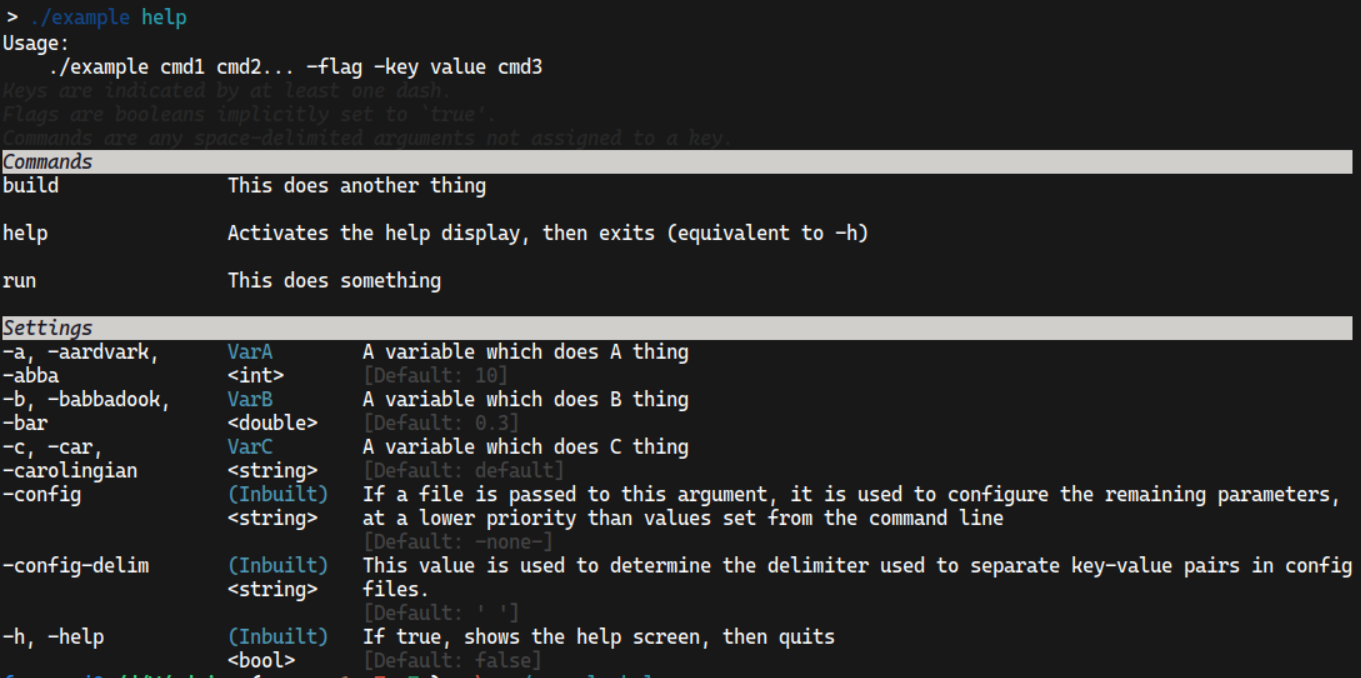
\includegraphics[width=\linewidth]{../media/help}
	\end{center}

	This is all generated automatically, without the user having to do anything, aside from add some useful comments to their code.


